\chapter{Modelo de Datos} \label{Anexo:ModeloDatos}
En este anexo se muestra el modelo de datos que modela el comportamiento de las clases actoras del juego. Toda clase actora hereda su comportamiento de una superclase llamada GameObject. Dentro del modelo de datos la tabla GameObject está compuesta de otras tablas que modelan componentes como máquina de estados para la animación, las dimensiones del GameObject, posición, etiqueta, el nivel donde aparece este GameObject y el colisionador. De esta tabla se especializan el resto de la tablas como Player, Moving Platform, etc. Dentro de las tablas especializadas hay casos como el de la tabla Horizontal Parol Enemy que es una especialización de la  tabla  Normal Enemy y está a su vez es una especialización de la tabla Enemy, misma que es una especialización de la tabla GameObject.
\begin{figure}[H]
    \centering
    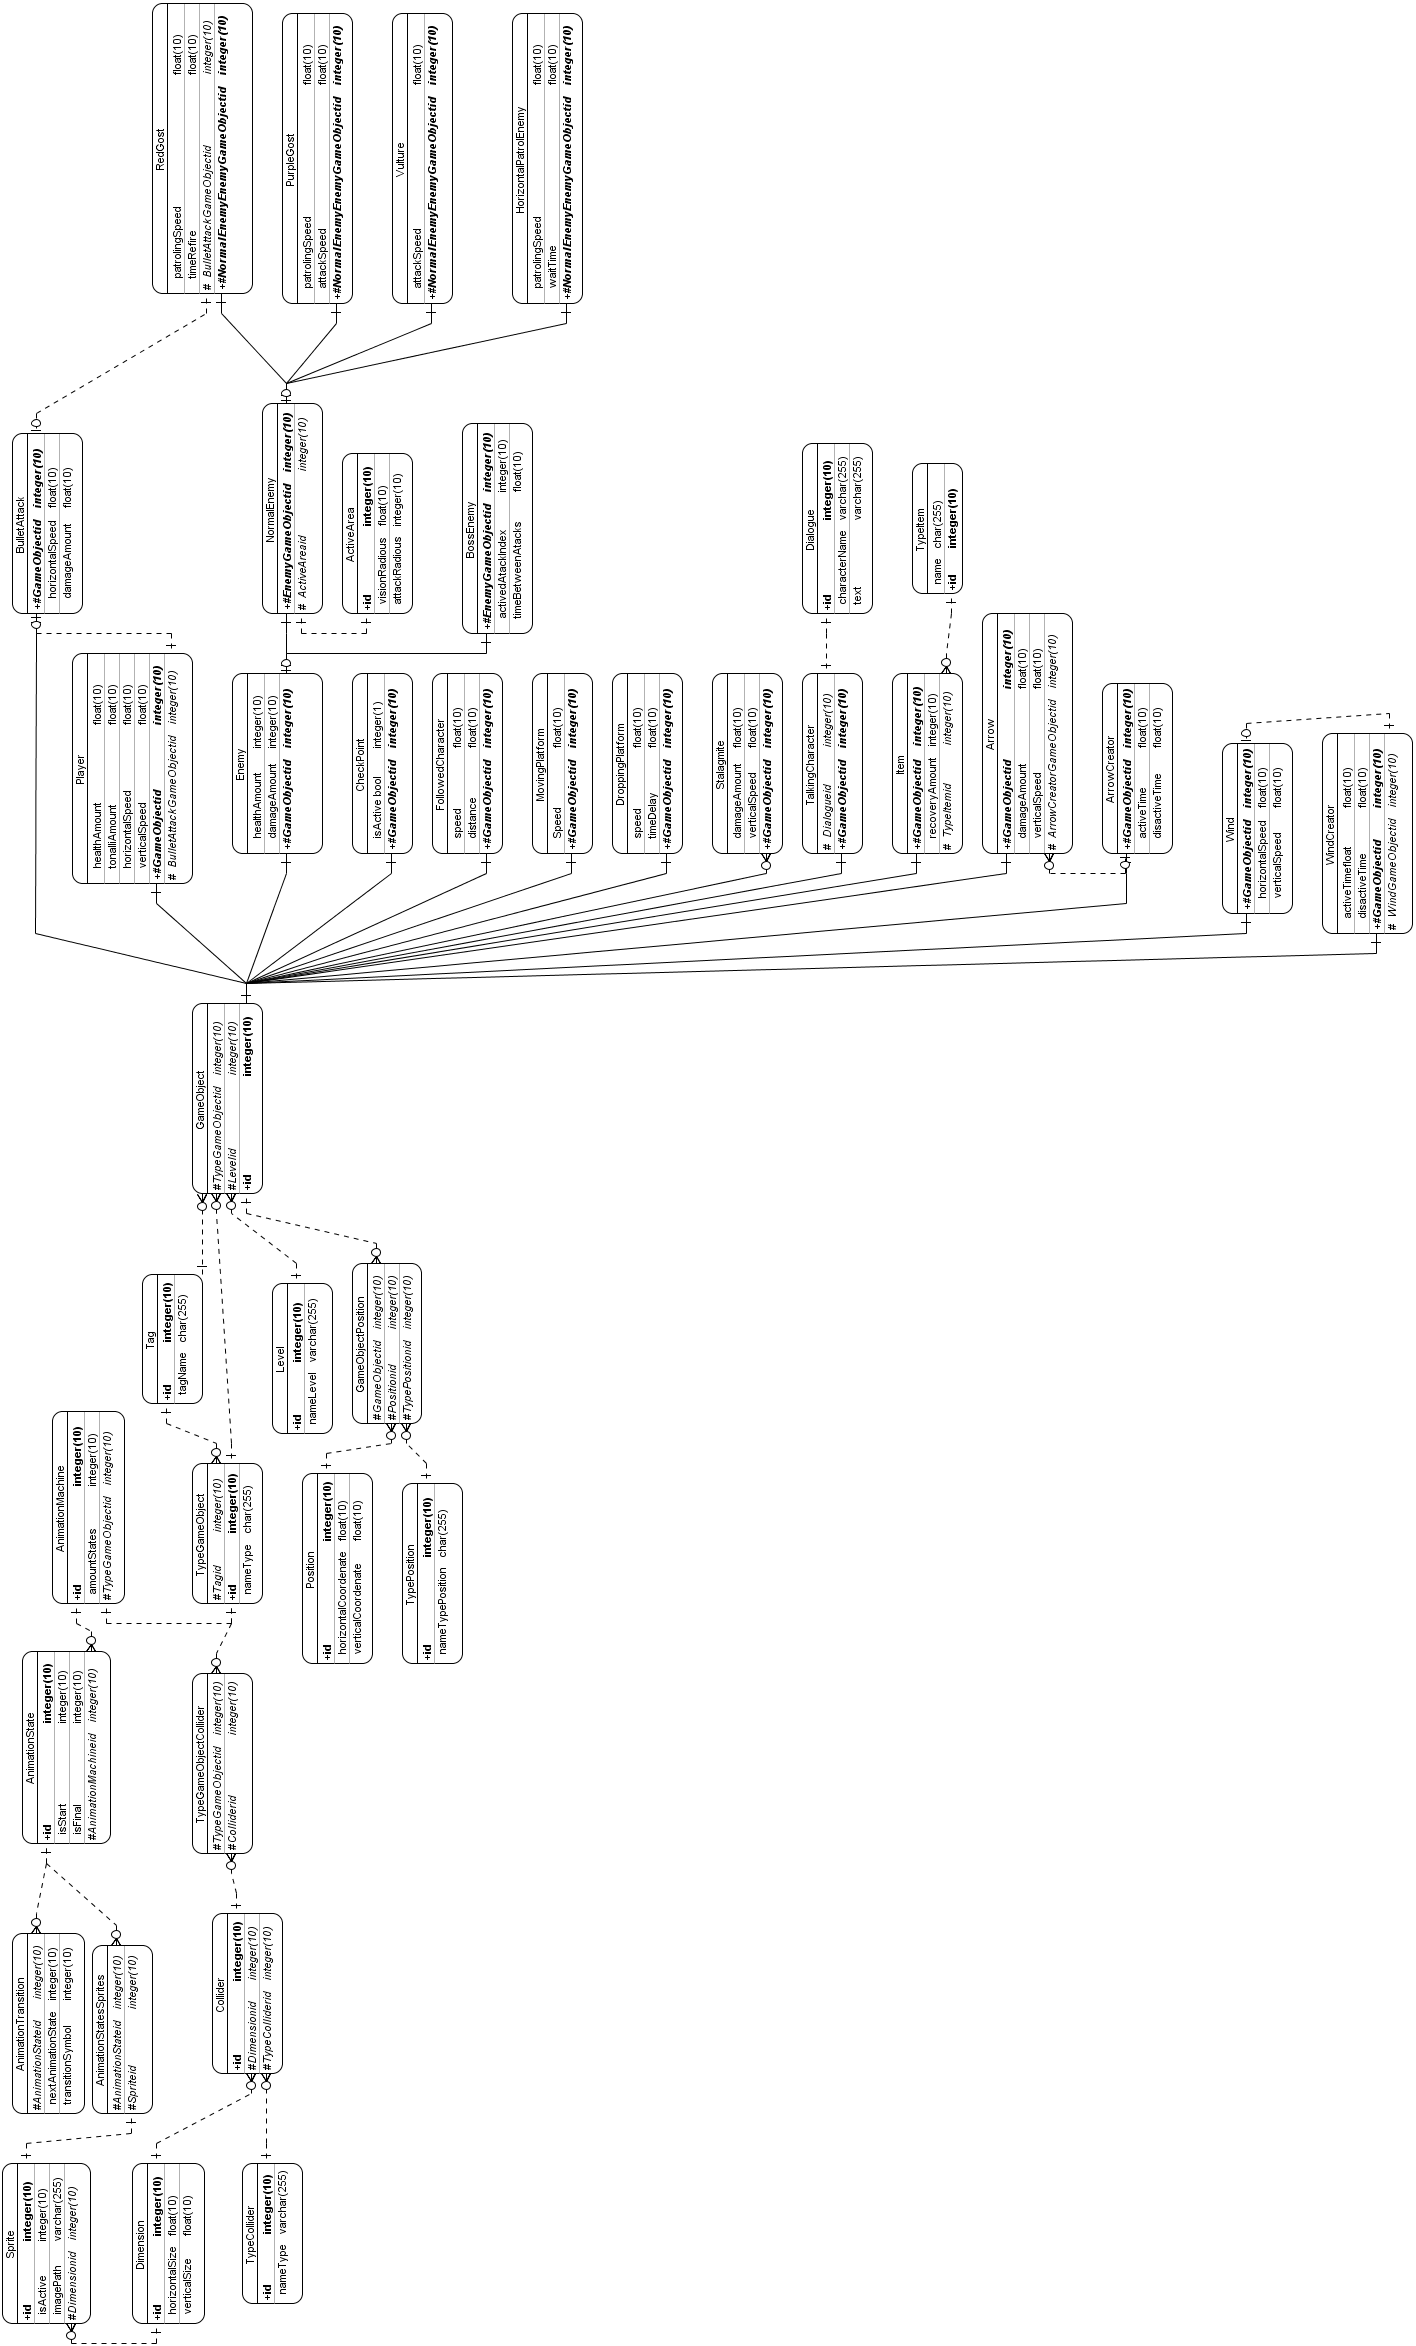
\includegraphics[width=0.75\textwidth]{Anexos/ModeloDatos/Yolotl02.png}
\end{figure}